%++++++++++++++++++++++++++++++++++++++++
% Don't modify this section unless you know what you're doing!
\documentclass[letterpaper,12pt]{article}
\usepackage{tabularx} % extra features for tabular environment
\usepackage{amsmath}  % improve math presentation
\usepackage{graphicx} % takes care of graphic including machinery
\usepackage[margin=1in,letterpaper]{geometry} % decreases margins
\usepackage{cite} % takes care of citations
\usepackage[final]{hyperref} % adds hyper links inside the generated pdf file
\hypersetup{
	colorlinks=true,       % false: boxed links; true: colored links
	linkcolor=blue,        % color of internal links
	citecolor=blue,        % color of links to bibliography
	filecolor=magenta,     % color of file links
	urlcolor=blue         
}
%++++++++++++++++++++++++++++++++++++++++


\begin{document}

\title{literature review : Fishing net simulations}
\author{A. Sarath krishnan, B. Partner, and C. Partner}
\date{\today}
\maketitle

\begin{abstract}
In this experiment we studied a very important physical effect by measuring the
dependence of a quantity $V$ of the quantity $X$ for two different sample
temperatures.  Our experimental measurements confirmed the quadratic dependence
$V = kX^2$ predicted by Someone's first law. The value of the mystery parameter
$k = 15.4\pm 0.5$~s was extracted from the fit. This value is
not consistent with the theoretically predicted $k_{theory}=17.34$~s. We attribute this
discrepancy to low efficiency of our $V$-detector.
\end{abstract}

%------------------------------------------------------------------------------------------------
\section{Chapter: works of E. Christensen and H. Chen}

\subsection{First Paper : Investigations on porous resistance coeffs for fishing net structures}

In the first paper which says about the investigations on the porous resistance coeffs, They have come up with an analytical solution for porous coeffs from physical parameters of fishing nets. Probably they might have modified the porous media flow solver in order to apply their approach in the simulation.  They have both Cm ( for inertial effect due to the presence of porous skelton) and S (resistance force) which consist of porous coeff matrices D and C. D comes in a linear term while C is in quadratic term which is the major part of the resistance force.
About neglecting D : This assumption was further justified by the physical explanation: Fishing nets are composed of twines with very small diameters, typical in the order of millimeters, the quadratic drag force is the dominant force for such kind of marine structures. Inertia and other forces are secondary.
Morison's equation and volume averaged NS for porous media are compared to find the equations for forces acting on the porous media. As morison's force model does not consider the interactions between nets, 2 coefficients a,b were introduced to predict the forces more accurately.Velocity inside porous media and undisturbed velocity have negligible difference and they are assumed to be same!
The equations involve angle of attacks and velocity directions. To implement this in a trawling nets could lead to edit the solver.

VALIDATION : The first validation case is based on the experimental data presented in Patursson (2007) for a plane net panel in current
flow under various attack angles and incoming velocities. ( A concern in velocity reduction from a porous baffle model if it is modeled as surface.! Will it provide the same velocity ( Even directions ) as the flow in reality? Stream lines will be deflecting near the net. But when we  make it as a porous surface, it wont right?)
validating with experiments by Zhan et al (2016) : Totally three kinds of net panels with different solidity ratios were studied in the experiments. The mesh for all the three nets were square diamond pattern. They calculated parameters for obtaining quadratic drag coeffs. Drag force was over predicted upto 40 percent  at 0.5 m/s and 30ª angle of attack. relative errors of most of the cases are less than 20 percent they say.
 Errors vary with different net cases : this shows a lack of good porous resistance coefficients ? for net 3, all drag forces were under estimated showing problems in coefficients a and b.
They have also done validations on current interactions with circular fish cages for aqua culture and wave interaction with net panels.
They carried out sensitivity analysis on porous resistance coeffs to know if they are in reasonable bounds when taking account uncertainties of numerical model. The uncertainties of the porous resistance coefficients come from the following: The drag force coefficient of the twines for a fishing net was assigned with a 10 percent uncertainty due to, i.e. misreading of the figure for drag force coefficients, difference between the shape of the real twine and a cylinder,etc. The projected area S1 and S2 for the in-plane and out-of-plane twines were varied with 5 percent, since they were usually calculated based on the mesh distance and the overall dimension of the fishing nets, therefore there exists round-off errors.
\subsection{Second paper : Development of a numerical model for fluid-structure interaction analysis
of flow through and around an aquaculture net cage}
More detailed paper on FSI for aquaculture net cages. A coupled problem was solved by porous media model for fluid and lumped mass structural solver with an efficient data exchange via RAM. The structural code was implemented inside the Pimple loop. A deforming mesh technique was used for representing rotating porous zone. A flow chart given for FSI. fluid model took more time than solid model. 

%----------------------------------------------------------------------------------------

\section{Vol 9 Contributions on the theory of fishing gears and related marine systems}

\subsection{The Hydrodynamic drag coeffs of flat netting at longitudinal flow - V.Naumov, N.Agievich}
Coefficient of hydrodynamic drag of a flat netting (Net parallel to the flow) depends on Reynolds number calculated by taking Length of the netting as characteristic length and \(omega\) : relation of threads area to projected area, and \(small delta\) : thickness on the thread to length of the netting. there exist three different areas of drag where Cd is proportional, inversely proportional and independent of Re(L)

considering the flow over a flat plate, since the netting is not really a hydro-dynamically smooth surface, roughness has to be considered. Ratio of $\Delta/l$ , where $\Delta$ is average irregularities and l is boundary layer thickness plays important role. As 'l' boundary layer thickness increases downstream, this ratio decreases.  so the front and rear will behave differently in terms of hydrodynamic resistance due to roughness.

Re1 : 2.4*10⁵ 
Re2 : 2*10⁶

when ReL less than Re1, inversely proportional to Cd by -0.16
when ReL between Re1 and Re2 proportional to Cd by a power of 0.14
ReL greater than Re2, independent of Rel 
They have provided the equations to find Cd for different velocities and compared it with some experiments conducted by other authors.
%------------------------------------------------------------------------------------------
\subsection{Impact of net shape and angle of attack on flow through net panel : Experimental study - christian Semlow, Mathias Paschen}
Purpose is to provide a validation data for CFD studies (Aquaculture). Hot wire probes and prandtl's tube where the sensors used to find the flow and pressure in the vicinity of the net.
Definition of porosity of the mesh : 
\begin{equation}
    \phi= 1 - \frac{d}{a}*\frac{1}{u_1*u_2}
\end{equation}
Where $u_1$ is the hanging ratio given by $sin\gamma$, $\gamma$ is the angle of arrangement of rhombic mesh. No information about $u_2$ is in the paper. ($u_2$ will be the hanging ratio in other direction.)
They notice a significant increase in velocity in the netting plane area compared to the undisturbed flow. the rate id velocity in the netting plane area corresponds to the porosity and is in accordance with continuity equation. Orientation of the net and hanging ratio have visible impact on velocity distribution.


%-------------------------------------------------------------------------------------------------
\section{Vol 8 : Contributions on theory of fishing gears and related marine systems}
\subsection{The hydrodynamic drag coeffs of flat netting at cross flow- V Naumov, N. Velicanov}
To find the drag coeff of flat netting when flow is parallel to the net. Old tries to find the analytical formula for drag coeffs are given. Inorder to find the critical Reynolds number, experiments are conducted for low Reynolds numbers. ($Re < 150$) The details regarding experimental set up used is given.
Theory of stochastic functions has been used for processing the experimental data. The formula to find the critical reynolds number's is given. Cd doesnot depend on reynolds number after Re is higher than higher limit critical value ReK. 






\section{Theory}

Here give a brief summary of the physical effect of interest and provide
necessary equations. Here is how you insert an equation. According to
references~\cite{melissinos, Cyr, Wiki} the dependence of interest is given
by
\begin{equation} \label{eq:aperp} % the label is used to reference the equation
u(\lambda,T)=\frac{8\pi hc\lambda^{-5}}{e^{hc/\lambda kT}-1},
\end{equation}
where T is temperature in Kelvin, c is the speed of light, etc. Don't forget to
explain what each variable means the first time that you introduce it.


\section{Procedures}

Give a schematic of the experimental setup(s) used in the experiment (see
figure~\ref{fig:samplesetup}). Give the description of  abbreviations
either in the figure caption or in the text. Write a description of what is
going on. 

\begin{figure}[ht] 
        % read manual to see what [ht] means and for other possible options
        \centering 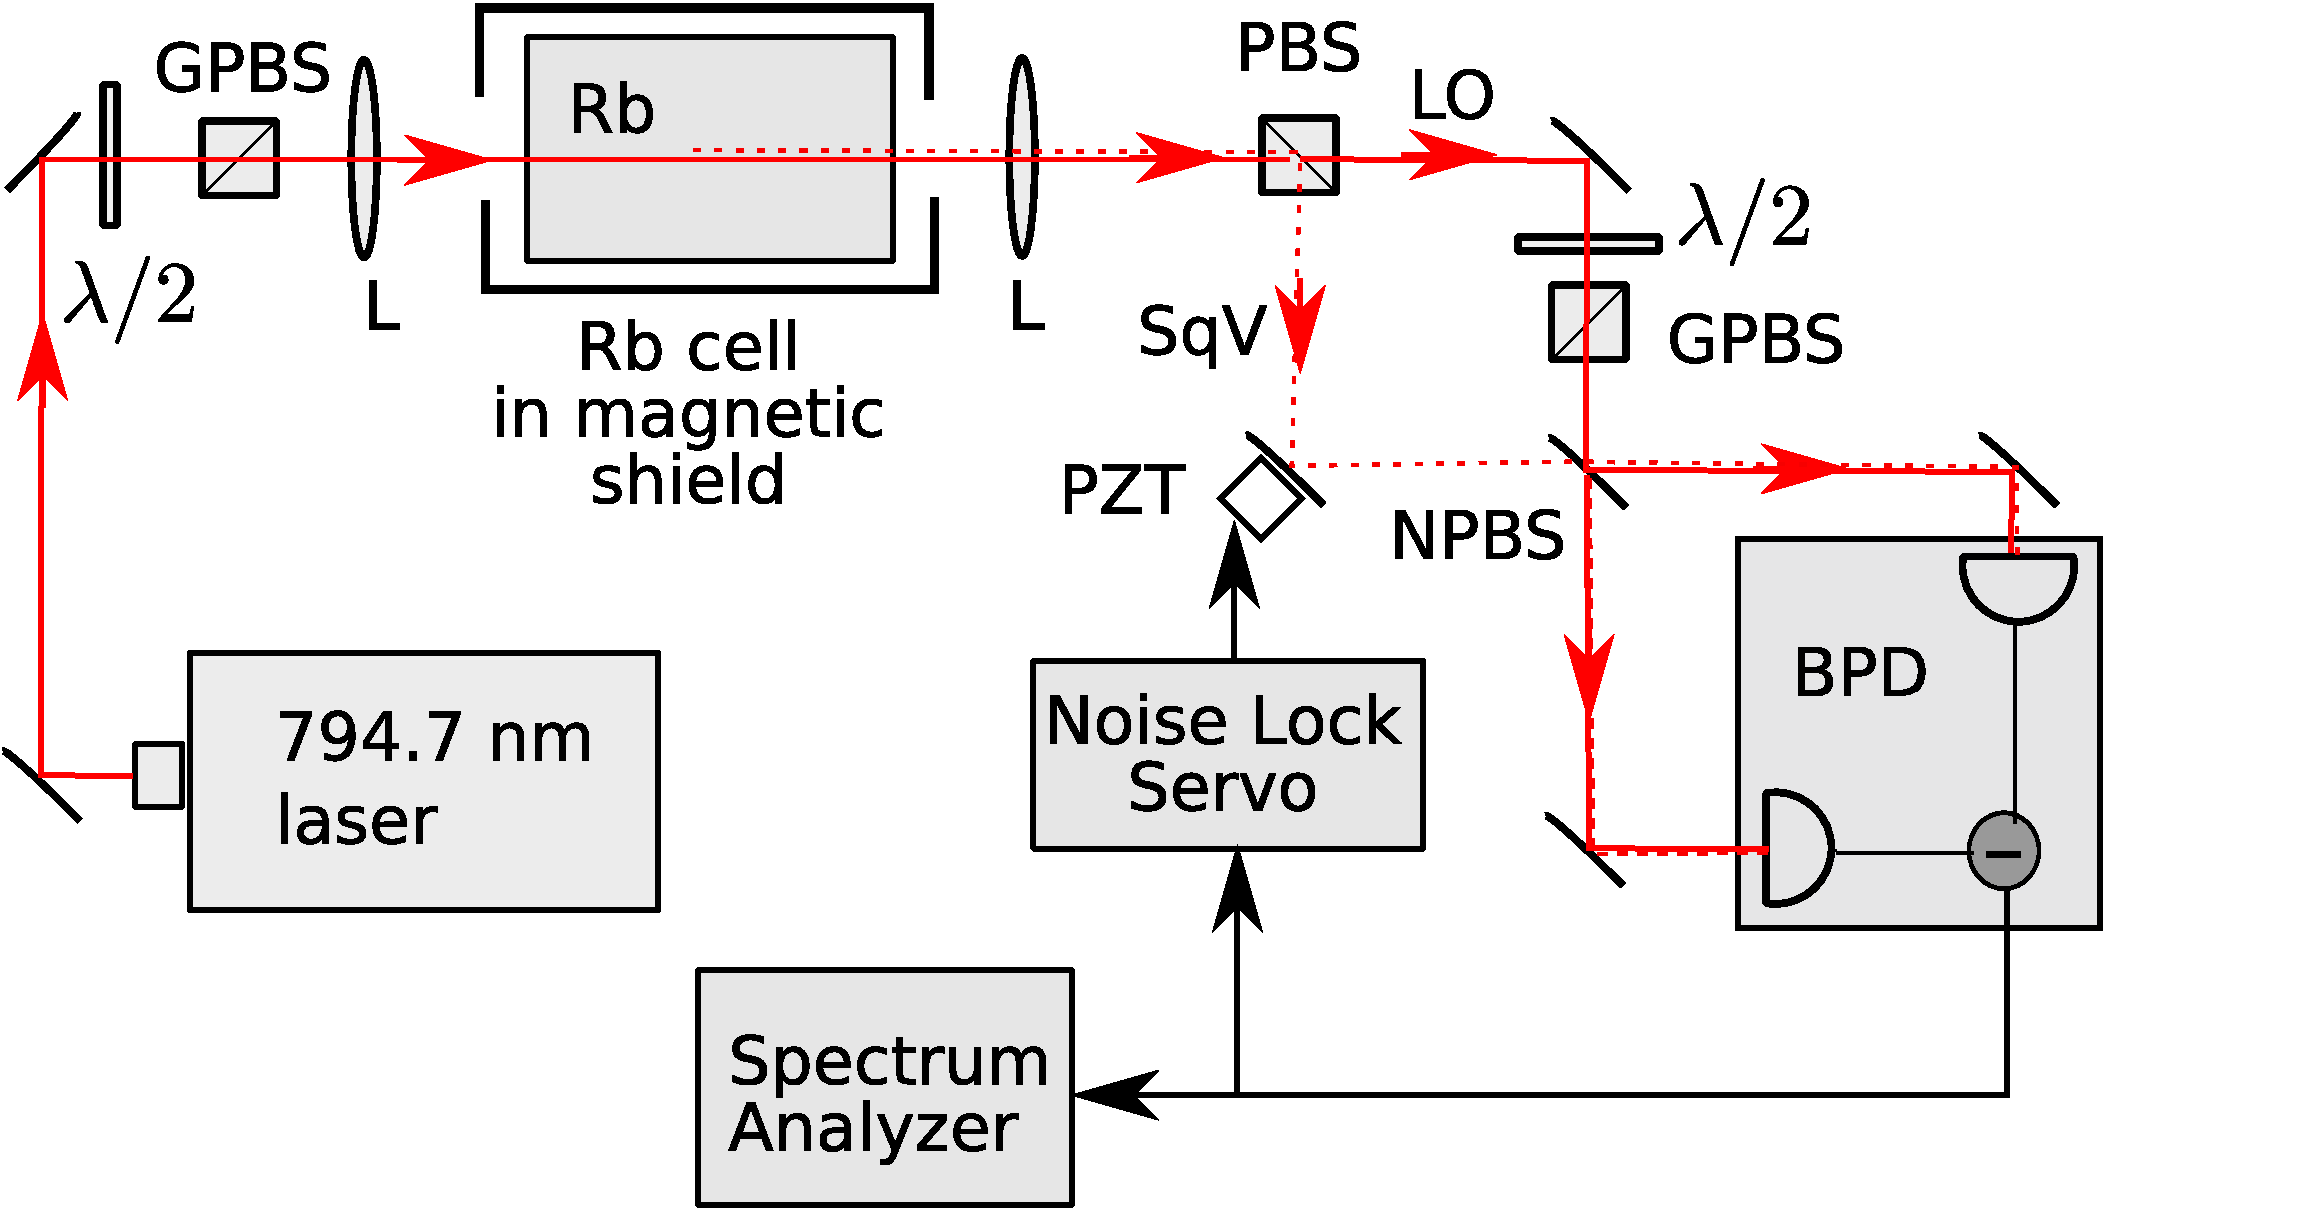
\includegraphics[width=0.8\columnwidth]{sr_setup}
        % note that in above figure file name, "sr_setup",
        % the file extension is missing. LaTeX is smart enough to find
        % apropriate one (i.e. pdf, png, etc.)
        % You can add this extention yourself as it seen below
        % both notations are correct but above has more flexibility
        %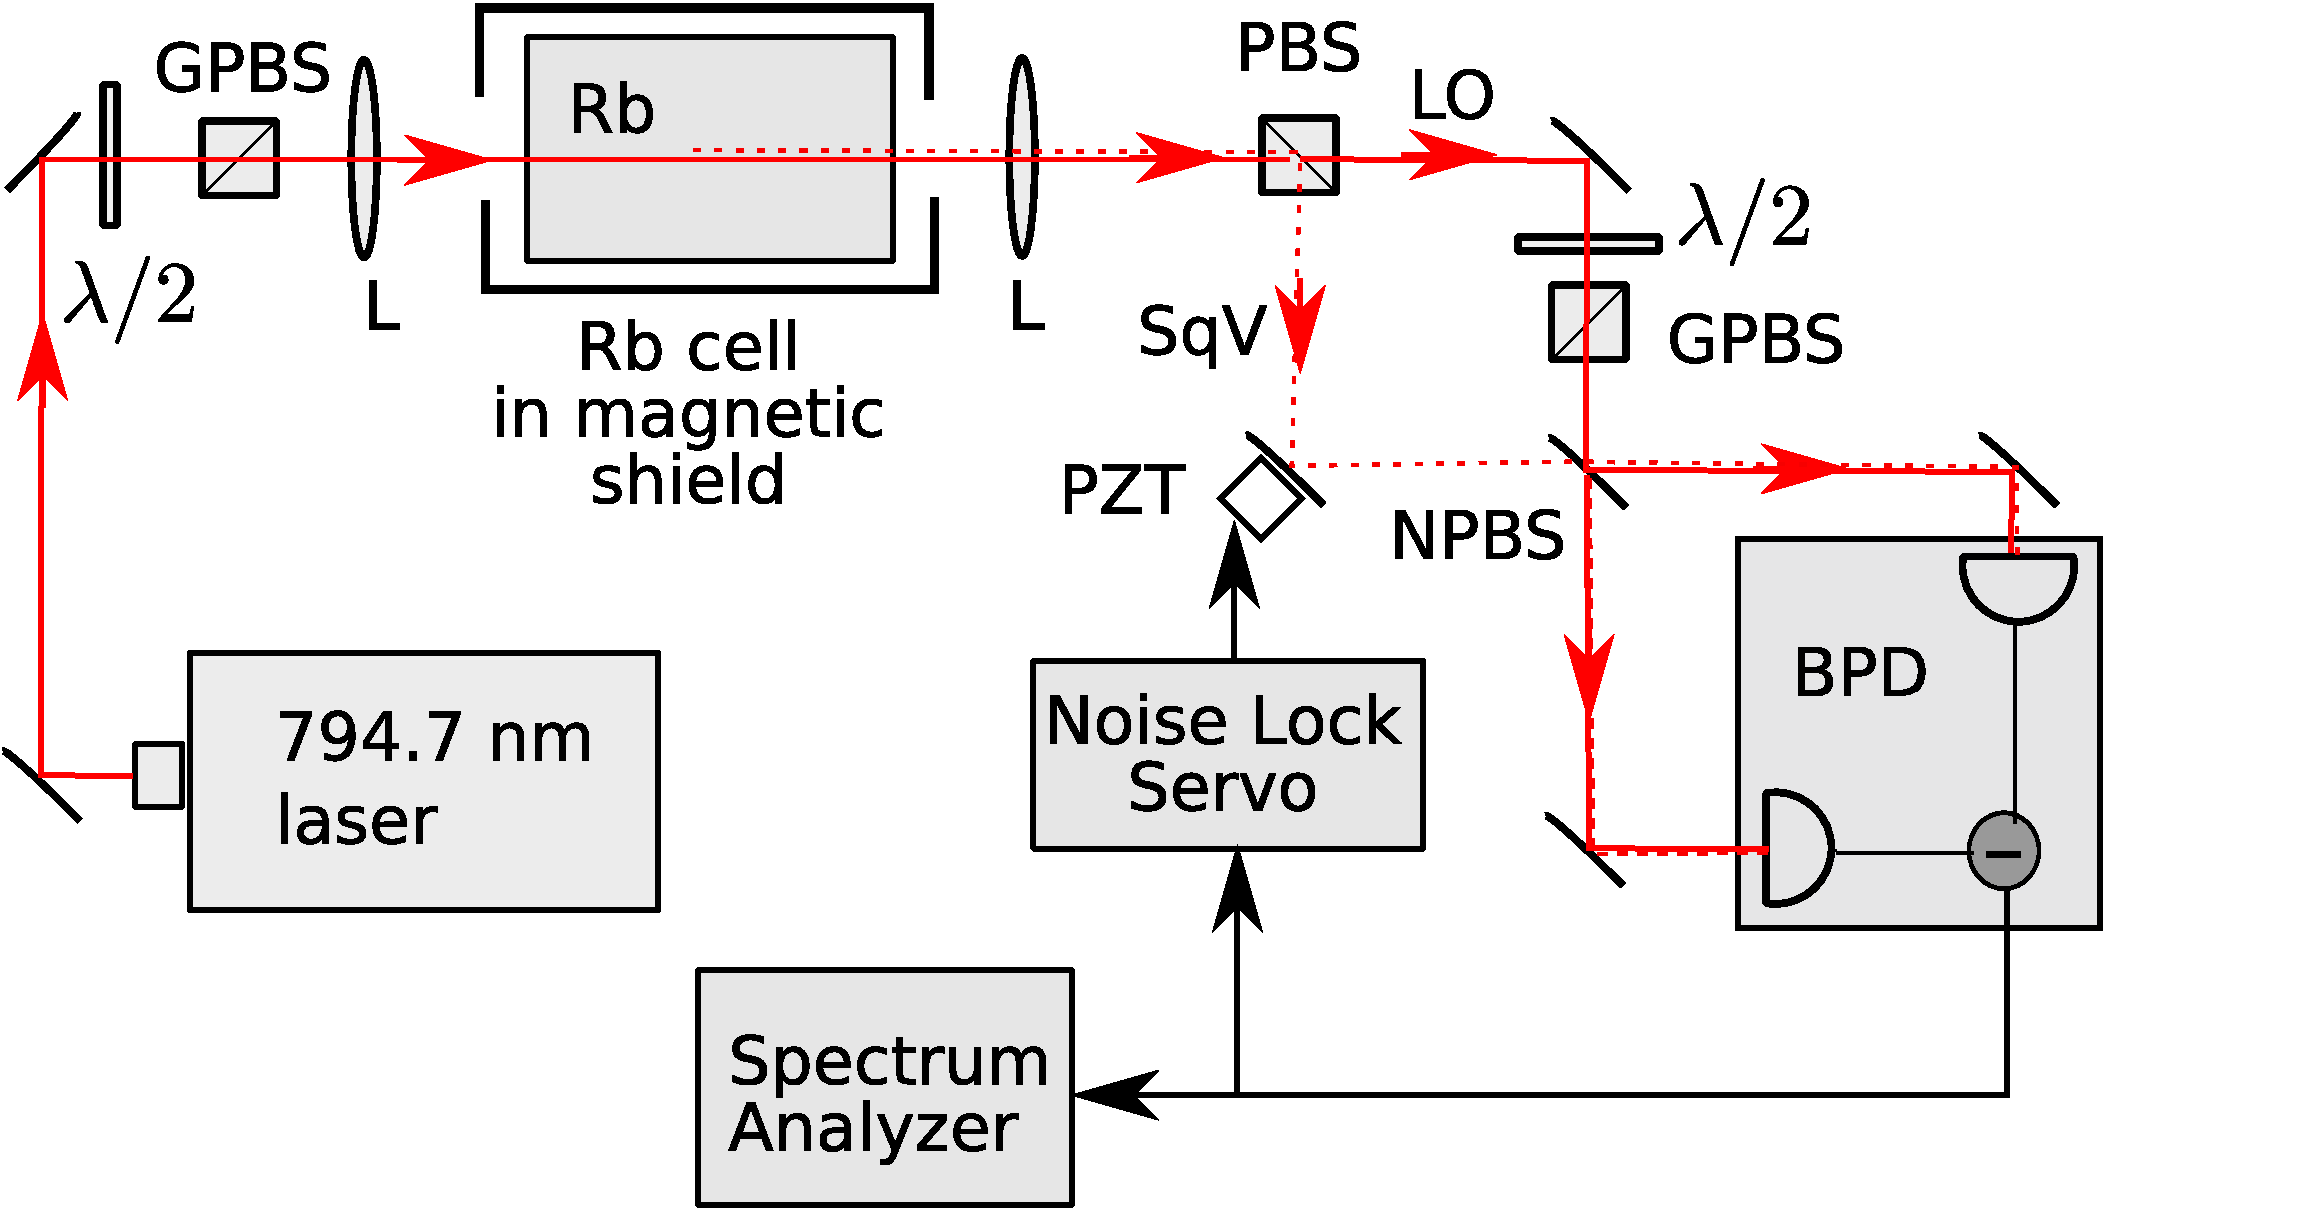
\includegraphics[width=1.0\columnwidth]{sr_setup.pdf}
        \caption{
                \label{fig:samplesetup} % spaces are big no-no withing labels
                % things like fig: are optional in the label but it helps
                % to orient yourself when you have multiple figures,
                % equations and tables
                Every figure MUST have a caption.
        }
\end{figure}

Don't forget to list all important steps in your experimental procedure!

Use active voice either in past or present through all the report and be
consistent with it:
The laser light comes  from to ... and eventually arrived to the
balanced photodiode as seen in the figure~\ref{fig:samplesetup}.

Sentences in the past voice while correct are generally considered hard to read
in large numbers. The laser light was directed to ..., wave plates were set
to ... etc.


\section{Analysis}

In this section you will need to show your experimental results. Use tables and
graphs when it is possible. Table~\ref{tbl:bins} is an example.

\begin{table}[ht]
\begin{center}
\caption{Every table needs a caption.}
\label{tbl:bins} % spaces are big no-no withing labels
\begin{tabular}{|cc|} 
\hline
\multicolumn{1}{|c}{$x$ (m)} & \multicolumn{1}{c|}{$V$ (V)} \\
\hline
0.0044151 &   0.0030871 \\
0.0021633 &   0.0021343 \\
0.0003600 &   0.0018642 \\
0.0023831 &   0.0013287 \\
\hline
\end{tabular}
\end{center}
\end{table}

Analysis of equation~\ref{eq:aperp} shows ...

Note: this section can be integrated with the previous one as long as you
address the issue. Here explain how you determine uncertainties for different
measured values. Suppose that in the experiment you make a series of
measurements of a resistance of the wire $R$ for different applied voltages
$V$, then you calculate the temperature from the resistance using a known
equation and make a plot  temperature vs. voltage squared. Again suppose that
this dependence is expected to be linear~\cite{Cyr}, and the proportionality coefficient
is extracted from the graph. Then what you need to explain is that for the
resistance and the voltage the uncertainties are instrumental (since each
measurements in done only once), and they are $\dots$. Then give an equation
for calculating the uncertainty of the temperature from the resistance
uncertainty. Finally explain how the uncertainty of the slop of the graph was
found (computer fitting, graphical method, \emph{etc}.)

If in the process of data analysis you found any noticeable systematic
error(s), you have to explain them in this section of the report.

It is also recommended to plot the data graphically to efficiently illustrate
any points of discussion. For example, it is easy to conclude that the
experiment and theory match each other rather well if you look at
Fig.~\ref{fig:samplesetup} and Fig.~\ref{fig:exp_plots}.

\begin{figure}[ht] 
  \centering
      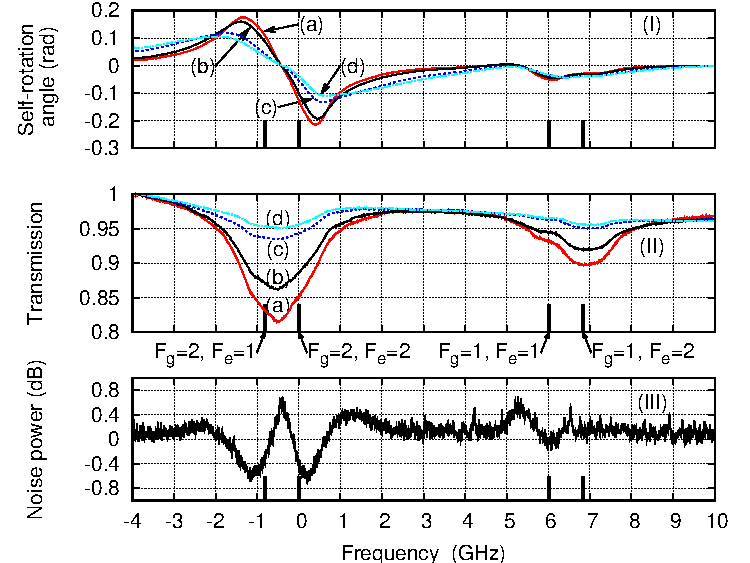
\includegraphics[width=0.5\columnwidth]{sr_squeezing_vs_detuning}

% some figures do not need to be too wide
        \caption{
                \label{fig:exp_plots}  
                Every plot must have axes labeled.
        }
\end{figure}


\section{Conclusions}
Here you briefly summarize your findings.

%++++++++++++++++++++++++++++++++++++++++
% References section will be created automatically 
% with inclusion of "thebibliography" environment
% as it shown below. See text starting with line
% \begin{thebibliography}{99}
% Note: with this approach it is YOUR responsibility to put them in order
% of appearance.

\begin{thebibliography}{99}

\bibitem{melissinos}
A.~C. Melissinos and J. Napolitano, \textit{Experiments in Modern Physics},
(Academic Press, New York, 2003).

\bibitem{Cyr}
N.\ Cyr, M.\ T$\hat{e}$tu, and M.\ Breton,
% "All-optical microwave frequency standard: a proposal,"
IEEE Trans.\ Instrum.\ Meas.\ \textbf{42}, 640 (1993).

\bibitem{Wiki} \emph{Expected value},  available at
\texttt{http://en.wikipedia.org/wiki/Expected\_value}.

\end{thebibliography}


\end{document}
